\documentclass{beamer}
\usepackage{amssymb}
\usepackage{amsmath}
\usepackage{mathtools}
\usepackage{enumerate}
\usepackage{esint}
\usepackage{siunitx}
\usepackage{bbm}
\usepackage{graphicx}
\usepackage{caption}
\usepackage{subcaption}
\usepackage{wrapfig}
\usepackage{epstopdf}
\usepackage{float}
\usepackage{cite}
\newcommand{\conj}[1]{\overline{#1}}
\newcommand{\newpar}{\vspace{5mm}\par}
\newcommand{\vnorm}[1]{\left\|#1\right\|}
\newcommand{\ket}[1]{\left\vert#1\right>}
\newcommand{\bra}[1]{\left<#1\right\vert}
\newtheorem{remark}{Remark}
\usepackage{amsthm}
\mode<presentation>{}
\usetheme{CambridgeUS}
\usepackage{tikz}
\usepackage{collcell}
\newtheorem{thm}{Theorem}
\newtheorem{prop}{Proposition}
\newtheorem{lem}{Lemma}
\usetikzlibrary{calc,arrows,quotes,angles}
\usepackage{arydshln}
\usetikzlibrary{shapes,snakes}
\usepackage{multicol}







\begin{document}
\title{Cometric Association Schemes}
\date[September 14, 2018]{PhD Thesis Proposal\\September 14, 2018}
\author{Brian Kodalen}
\institute[WPI]{Worcester Polytechnic Institute}
\frame{\titlepage}

\begin{frame}
	\tableofcontents
\end{frame}

\section{Association schemes}
\begin{frame}
	\frametitle{Symmetric Association Scheme}
	A \textbf{symmetric association scheme} is an ordered pair $(X,\mathcal{R})$ where $X$ is a finite set and $\mathcal{R} = \left\{R_0,\dots,R_d\right\}$ is a partition of $X\times X$ into $d+1$ symmetric binary relations satisfying
	\begin{itemize}
		\item $R_0$ is the identity relation on $X$
		\item for $0\leq i,j,k\leq d$, there exists $p^k_{ij}\in\mathbb{Z}$ such that
		\[\vert R_i(a)\cap R_j(b)\vert = p^k_{ij}\]
		whenever $(a,b)\in R_k$.
	\end{itemize}
\end{frame}

\begin{frame}
\frametitle{Example: Heawood Graph}
\centering
\scalebox{.9}{\begin{tikzpicture}[shorten >=1pt,auto,node distance=2cm,
thin,main node/.style = {circle,draw, minimum size = 5pt}]
\def\r{3.5}
\foreach \t in {0,...,13}
{{\node[main node] at ({\r*cos(180*(1+\t / 7))},{\r*sin(180*(\t / 7))}) (\t) {\t};}
{\node[main node] at ({\r*cos(180*(1+\t / 7))},{\r*sin(180*(\t / 7))}) (\t) {\t};}}
\draw[-] (13)--(0)--(1)--(2)--(3)--(4)--(5)--(6)--(7)--(8)--(9)--(10)--(11)--(12)--(13);
\draw[-] (0)--(5)--(4)--(9)--(8)--(13)--(12)--(3)--(2)--(7)--(6)--(11)--(10)--(1);
%base
\only<2->{
\foreach \t in {0}
{{\node[main node] at ({\r*cos(180*(1+\t / 7))},{\r*sin(180*(\t / 7))}) (\t) {\t};}
	{\node[main node,fill=blue] at ({\r*cos(180*(1+\t / 7))},{\r*sin(180*(\t / 7))}) (\t) {\t};}}}
%distance 1
\only<3->{
\foreach \t in {1,5,13}
{{\node[main node] at ({\r*cos(180*(1+\t / 7))},{\r*sin(180*(\t / 7))}) (\t) {\t};}
	{\node[main node,fill=red] at ({\r*cos(180*(1+\t / 7))},{\r*sin(180*(\t / 7))}) (\t) {\t};}}}
%distance 2
\only<4->{
\foreach \t in {2,10,12,8,4,6}
{{\node[main node] at ({\r*cos(180*(1+\t / 7))},{\r*sin(180*(\t / 7))}) (\t) {\t};}
	{\node[main node,fill=green] at ({\r*cos(180*(1+\t / 7))},{\r*sin(180*(\t / 7))}) (\t) {\t};}}}
%distance 3
\only<5->{
\foreach \t in {3,7,9,11}
{{\node[main node] at ({\r*cos(180*(1+\t / 7))},{\r*sin(180*(\t / 7))}) (\t) {\t};}
	{\node[main node,fill=yellow] at ({\r*cos(180*(1+\t / 7))},{\r*sin(180*(\t / 7))}) (\t) {\t};}}}
\end{tikzpicture}}
\end{frame}

\begin{frame}
\frametitle{Bose-Mesner Algebra}
Let $A_i$ denote the adjacency matrix of the graph $(X,R_i)$.
\[\mathbb{A} = \text{span}_\mathbb{R}(A_0,A_1,\dots,A_d)\]
\begin{itemize}
	\item commutative algebra of symmetric matrices;
	\item closed under entrywise products.
\end{itemize}
\vfill
Second basis using idempotents:
\[\mathbb{A} = \text{span}_\mathbb{R}(E_0,E_1,\dots,E_d)\]

\end{frame}




\begin{frame}
\frametitle{Polynomial Schemes}
$(X,\mathcal{R})$ is {\em$P$-polynomial} ({\em metric}) if we can order the relations so that:
\[p^k_{ij}\begin{cases}
= 0, & k>i+j \text{ or } k<\vert i-j\vert\\
\neq 0, & k = i+j
\end{cases}\]
Examples
\begin{multicols}{2}
	\begin{itemize}
	\item SRGs
	\item Generalized Quadrangles
	\item Projective Planes
	\end{itemize}
\end{multicols}
\end{frame}

\begin{frame}
\frametitle{Q-polynomial}
$(X,\mathcal{R})$ is {\em $Q$-polynomial} if we can order the idempotents so that:
\[q^{k}_{ij} = \begin{cases}
0 & k>i+j\text{ or }k<\vert i-j\vert\\
>0 & k = i+j\\
\end{cases}\]
$\mathcal{A}$ is \textit{Q-antipodal} if $q^{k}_{dd}>0 \iff k\in\left\{0,d\right\}$

\end{frame}

\section{Connectivity}
\section{Linked simplices}
\section{Sch\"{o}nberg's theorem}

\end{document}


\section{Linked simplices}
\subsection*{test}
\begin{frame}
\frametitle{(real) Mutually Unbiased Bases}
A set of $w$ orthonormal bases of $\mathbb{R}^n$ such that
\[\left<a,b\right> = \pm\frac{1}{\sqrt{n}}\]
whenever $a$ and $b$ are from distinct bases.\\\pause
\vfill
What is the maximum size, $M(n)$, of a set of MUBs in $\mathbb{R}^n$?
\begin{itemize}
	\item 30 year old problem. (Ivonovic `81, Wootters \& Fields `89)
	\item $M(n)>1$ only if $n=4t$ for some $t\in\mathbb{N}$. (Boykin et.\ al.\ `08)
	\item $M(n)\leq n/2+1$. (Delsarte, Goethals, Seidel `75)
	\item Tight examples exist whenever $n = 4^t$. (Cameron, Seidel `73)
\end{itemize}
\end{frame}
\begin{frame}
	\frametitle{(real) Equiangular Lines}
A set of $w$ vectors in $\mathbb{R}^n$ such that
\[\left<a,b\right> = \pm \alpha\]
for fixed $\alpha$ whenever $a\neq b$.\\\pause
\vfill
What is the maximum size, $N(n)$, of a set of equiangular lines in $\mathbb{R}^n$?
\begin{itemize}
	\item 70 year old problem. (Haantjes `48)
	\item Closely related to graphs. (Van Lint \& Seidel `66)
	\item $N(n)\leq\binom{n+1}{2}$. (Gerzon `71)
	\item If $N(n)>2n$, $\frac{1}{\alpha}$ is an odd integer. (Neumann `71)
\end{itemize}
\end{frame}

\begin{frame}
\begin{columns}
	\begin{column}{0.7\textwidth}
	\frametitle{Two simplices in $\mathbb{R}^2$}
	\[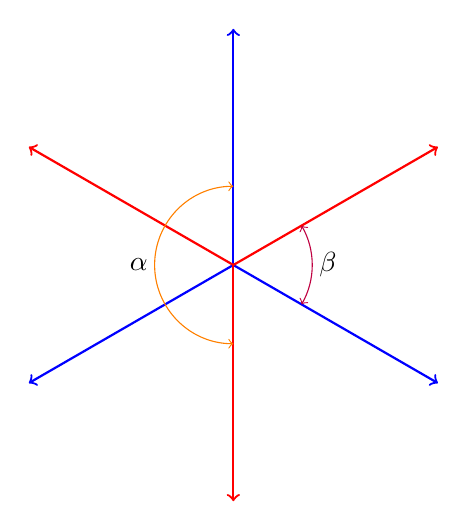
\begin{tikzpicture}
		\coordinate (a) at (0,0);
		\coordinate (b) at (0,3);
		\coordinate (c) at (0,-3);
		\coordinate (d) at ($(0,-3/2) + sqrt(3)*(3/2,0)$);
		\coordinate (e) at ($(0,3/2) + sqrt(3)*(3/2,0)$);
		
		\draw[blue,->,thick] (0,0) -> (0,3);
		\draw[blue,->,thick] (0,0) -> ($(0,-3/2) + sqrt(3)*(3/2,0)$);
		\draw[blue,->,thick] (0,0) -> ($(0,-3/2) + sqrt(3)*(-3/2,0)$);\pause
		\draw[red,->,thick] (0,0) -> (0,-3);
		\draw[red,->,thick] (0,0) -> ($(0,3/2) + sqrt(3)*(3/2,0)$);
		\draw[red,->,thick] (0,0) -> ($(0,3/2) + sqrt(3)*(-3/2,0)$);\pause
		\draw pic["$\alpha$",draw=orange,<->,angle eccentricity=1.2,angle radius=1cm] {angle=b--a--c};
		\draw pic["$\beta$",draw=purple,<->,angle eccentricity=1.2,angle radius=1cm] {angle=d--a--e};
	\end{tikzpicture}\]
	\end{column}
	\begin{column}{0.3\textwidth}
	\only<3->{
	\[\begin{aligned}
	\alpha &= 180^\circ\\
	\beta &= 60^\circ\\\\
	\left<\text{red},\text{blue}\right>&\in\left\{-1,\frac{1}{2}\right\}
	\end{aligned}\]}
	\end{column}
\end{columns}
\end{frame}

\begin{frame}
\frametitle{Two simplices in $\mathbb{R}^3$}
\begin{columns}
	\begin{column}{0.7\textwidth}
		\[\begin{tikzpicture}[line join = round, line cap = round]
		
		\coordinate (a) at (0,0,0);
		\pgfmathsetmacro{\factor}{1/sqrt(2)};
		\coordinate (A) at (2,0,-2*\factor);
		\coordinate (B) at (-2,0,-2*\factor);
		\coordinate (C) at (0,2,2*\factor);
		\coordinate (D) at (0,-2,2*\factor);
		
		\draw[->] (0,0) -- (3,0,0) node[right] {$x$};
		\draw[->] (0,0) -- (0,3,0) node[above] {$y$};
		\draw[->] (0,0) -- (0,0,3) node[below left] {$z$};
		\foreach \i in {A,B,C,D}
		\draw[thick,blue,->] (0,0)--(\i);
		\only<1>{\draw[-,dashed, fill=blue!30, opacity=.2] (A)--(C)--(B)--cycle;
		\draw[-,dashed, fill=red!30, opacity=.2] (A) --(D)--(C)--cycle;
		\draw[-,dashed, fill=purple!30, opacity=.2] (B)--(D)--(C)--cycle;}\pause
		
		
		\coordinate (A1) at (-2,0,2*\factor);
		\coordinate (B1) at (2,0,2*\factor);
		\coordinate (C1) at (0,-2,-2*\factor);
		\coordinate (D1) at (0,2,-2*\factor);
		\foreach \i in {A1,B1,C1,D1}
		\draw[thick,red,->] (0,0)--(\i);
		\only<2>{\draw[-,dashed, fill=blue!30, opacity=.2] (A1)--(C1)--(B1)--cycle;
		\draw[-,dashed, fill=red!30, opacity=.2] (A1) --(D1)--(C1)--cycle;
		\draw[-,dashed, fill=purple!30, opacity=.2] (B1)--(D1)--(C1)--cycle;}\pause
		\draw pic["$\beta$",draw=orange,<->,angle eccentricity=1.2,angle radius=0.7cm] {angle=A--a--D1};
		\draw pic["$\alpha$",draw=purple,<->,angle eccentricity=1.2,angle radius=1cm] {angle=D1--a--D};
		\end{tikzpicture}\]
	\end{column}
	\begin{column}{0.3\textwidth}
		\only<3->{
			\[\begin{aligned}
			\alpha &= 180^\circ\\
			\beta &\approx 70.5^\circ\\\\
			\left<\text{red},\text{blue}\right>&\in\left\{-1,\frac{1}{3}\right\}
			\end{aligned}\]}
	\end{column}
\end{columns}
\end{frame}

\begin{frame}
\frametitle{Linked Simplices}
Regular simplex:
\begin{itemize}
	\item $v$ unit vectors spanning $\mathbb{R}^{v-1}$;
	\item pairwise inner products of $-\frac{1}{v-1}$.
\end{itemize}\pause
\vfill
Simplices $A$ and $B$ are ``linked" if there exists $\gamma,\delta\in\mathbb{R}$ with:
\[\forall (a,b)\in A\times B: \left<a,b\right> \in\left\{\gamma,\delta\right\}\]\pause
\vfill
Simplices $A_1,\dots,A_w$ are ``linked" if every pair is linked using the same constants.
\end{frame}

\begin{frame}
\frametitle{Two simplices in $\mathbb{R}^{v-1}$}
\begin{itemize}
	\item Let $A$ be a regular simplex in $\mathbb{R}^{v-1}$;
	\item let $A' = \left\{-a : a\in A\right\}$.
\end{itemize}
For each $a\in A$ and $a'\in A'$,
\[\left<a,a'\right> \in\left\{-1,\frac{1}{v}\right\}\]
\vfill\pause
Can you find 3 linked simplices?\\\pause
Can you find 2 without using -1 as an inner product?
\end{frame}


\begin{frame}
\frametitle{Pair of Linked Simplices}
\begin{thm}[K. `18]
	Let $\left\{a_i\right\}$ and $\left\{b_j\right\}$ be linked simplices with inner products $\gamma$ and $\delta$. Let $B_j = \left\{a_i: \left<a_i,b_j\right> = \gamma\right\}$. Then $(\left\{a_i\right\},\left\{B_j\right\})$ forms a $(v,k,\lambda)$ symmetric 2-design where $k$ and $\lambda$ depend only $\gamma$ and $\delta$.
\end{thm}\pause
\begin{thm}[K. `18]
	Let $A_1,\dots,A_w$ be $w$ linked simplices with inner products $\gamma$ and $\delta$. Define graph $\Gamma(X,E)$ on $X = \cup_i A_i$ and $E$ given by:\vspace{-.8em}
	\[\text{For }x\in A_i, y\in A_{i'}\quad (i\neq i'):\qquad x\sim y \iff \langle x,y\rangle = \gamma.\]
	Then $\Gamma(X,E)$ is a linked system of symmetric designs.
%\begin{enumerate}[(i)]
%\item For $x,y\in\mathbb{R}^{v-1}: %\sum_{i=1}^{v}\left<a_i,x\right>\left<a_i,y\right> = \frac{v}{v-1}\left<x,y\right>$;
%\end{enumerate}
\end{thm}
\end{frame}


\begin{frame}
\frametitle{Linked system of symmetric designs}
\begin{definition}[Cameron `72]
	A \textit{linked system of symmetric designs} ($LSSD(v,k,\lambda;w)$, $w\geq 2$) is a ($w$-partite) graph $\Gamma$ on $wv$ vertices with the following properties:\vspace{-.5em}
	\begin{enumerate}[(i)]
		\item $X = \dot{\cup}_{i=1}^wX_i$ with $\vert X_i\vert = v$;
		\item no edge of $\Gamma$ has both ends in the same fiber;\pause
		\item the induced subgraph between distinct fibers is the incidence graph of a $(v,k,\lambda)$-design;\pause
		\item there exist constants $\mu$ and $\nu$ such that for distinct $h,i,j$:
		\vspace{-.5em}\[a\in X_i,b\in X_j\rightarrow\vert \Gamma(a)\cap \Gamma(b)\cap X_h\vert = \begin{cases}
		\mu & a\sim b\\
		\nu & a\not\sim b.\\
		\end{cases}\]
		\vfill
	\end{enumerate}
\end{definition}
\end{frame}

\begin{frame}
	\frametitle{(iv) visualized}
	\[\begin{tikzpicture}[shorten >=1pt,auto,node distance=2cm,
	thin,main node/.style = {circle,draw, inner sep = 2pt},main2 node/.style = {circle,draw, inner sep = 1pt},vertex/.style = {circle, draw, fill, inner sep = 0pt, minimum size=2pt}]
		
		
		\node at (-.3,1) {$X_1$};
		\node at (5.3,1) {$X_2$};
		\node at (2.5,-3.5) {$X_3$};
		\draw (2.5,-2.5) ellipse (1.5cm and .7cm);
		\draw[rotate=30] (0,0) ellipse (1.5cm and .7cm);
		\draw[rotate around={-30:(5,0)}]  (5,0) ellipse (1.5cm and .7cm);;
		\node[vertex,label = 90:x](x) at (0,0) {};
		\node[vertex,label = 90:y](y) at (5,0) {};
		\draw[dashed] (x) -- (y);
		
		\only<2->{\draw[semithick] (x) -- (1.6,-2.55);
		\draw[semithick] (x) -- (2.4,-2.15);
		\draw[semithick] (2.2,-2.5) ellipse (.6 and .4);}
		
		
		
		\only<2->{\draw[semithick] (2.8,-2.5) ellipse (.6 and .4);
		\draw[semithick] (y) -- (2.6,-2.15);
		\draw[semithick] (y) -- (3.38,-2.55);}
	
		\only<3->{\node at (2.5,-2.5) {S};}
	\end{tikzpicture}\]
	\only<4->{\[\vert S\vert = \begin{cases}
		\mu & x\sim y\\
		\nu & x\not\sim y\\
		\end{cases}\]}
\end{frame}

\begin{frame}
\frametitle{Three Linked Simplices}
Given simplices: $\left\{a_i\right\}$, $\left\{b_j\right\}$, $\left\{c_\ell\right\}$:
 \vspace{-.7em}\[\begin{aligned}x_j &= \left[\left<a_1,b_j\right>,\left<a_2,b_j\right>,\dots,\left<a_v,b_j\right>\right]\\
 y_\ell &= \left[\left<a_1,c_\ell\right>,\left<a_2,c_\ell\right>,\dots,\left<a_v,c_\ell\right>\right]
 \end{aligned}\]\vfill\pause
 Let $\eta_{j\ell} = \vert\left\{a_i : \langle a_i,b_j\rangle = \langle a_i,c_\ell\rangle = \gamma \right\}\vert$.
  \vspace{-.5em}
 \[\begin{aligned}
 \langle x_j,y_\ell\rangle &= (\eta_{j\ell})\gamma^2 + 2(k-\eta_{j\ell})\gamma\delta + (v-2k+\eta_{j\ell})\delta^2 \end{aligned}\]\vfill\pause
 A regular simplex is a tight frame, so:\vspace{-.5em}
\[\langle x_j,y_\ell\rangle = \sum_i\langle a_i,b_j\rangle\langle a_i,c_\ell\rangle = \frac{v}{v-1}\langle b_j,c_\ell\rangle
\]\vfill\pause
\end{frame}

\section{Association schemes/LSSDs}
\subsection*{test2}

\begin{frame}
\frametitle{Symmetric association scheme}
	$\mathcal{A}=(X,\mathcal{R})$ with finite set $X$ and symmetric relations $\mathcal{R} = \left\{R_0,R_1,\dots,R_d\right\}$ on $X$ satisfying:
	\begin{itemize}
		\item $R_0$ is the identity relation.
		\item $\mathcal{R}$ is a partition of $X\times X$.
		\item There exist integers $p_{ij}^k$ such that 
		\[\vert \left\{z\in X:(x,z)\in R_i, (z,y)\in R_j\right\}\vert = p^k_{ij}\]
		whenever $(x,y)\in R_k$.
	\end{itemize}
\end{frame}



\begin{frame}
\frametitle{3-class $Q$-antipodal association schemes}
\begin{theorem}[Van Dam `99]
Let $\Gamma$ be a $LSSD$ with adjacency matrix $A$. The algebra $\left<A\right>$ is the Bose-Mesner algebra of a 3-class Q-antipodal association scheme. Conversely, every 3-class Q-antipodal association scheme arises in this way.
\end{theorem}
\end{frame}


\begin{frame}
	\frametitle{First and Second Eigenmatrices}
	\[\begin{aligned}P &= \left[\begin{array}{cccc}
	1 & k(w-1) & v-1 & (v-k)(w-1)\\
	1 & \sqrt{k-\lambda}(w-1) & -1 & -\sqrt{k-\lambda}(w-1)\\
	1 & -\sqrt{k-\lambda} & -1 & \sqrt{k-\lambda}\\
	1 & -k & v-1 & k-v\\
	\end{array}\right]\\
	\only<1>{Q&=\left[\begin{array}{cccc}
	1 & v-1 & (w-1)(v-1) & w-1\\
	1 & \frac{v-k}{\sqrt{k-\lambda}} & -\frac{v-k}{\sqrt{k-\lambda}} & -1\\
	1& -1 & 1-w & w-1\\
	1 & -\frac{k}{\sqrt{k-\lambda}} & \frac{k}{\sqrt{k-\lambda}} & -1
	\end{array}\right]}
	\only<2>{Q&=\left[\begin{array}{c|c|cc}
		\cline{2-2}
	1 &  v-1  & (w-1)(v-1) & w-1\\
	1 &  \frac{v-k}{\sqrt{k-\lambda}}  & -\frac{v-k}{\sqrt{k-\lambda}} & -1\\
	1&  -1  & 1-w & w-1\\
	1 &  -\frac{k}{\sqrt{k-\lambda}}  & \frac{k}{\sqrt{k-\lambda}} & -1\\
	\cline{2-2}
	\end{array}\right]}
	\end{aligned}\]
\end{frame}

\begin{frame}
\frametitle{Gram matrix}
%Let $\gamma = \frac{v-k}{(v-1)\sqrt{k-\lambda}}$ and $\delta = -\frac{k}{(v-1)\sqrt{k-\lambda}}$.
\[cE_1 = \left[\begin{array}{c:c:c}
\begin{smallmatrix}
1 & &-\frac{1}{v-1}\\
& \ddots &\\
-\frac{1}{v-1} & & 1
\end{smallmatrix} & \gamma,\delta &\gamma,\delta\\\hdashline
\gamma,\delta& \begin{smallmatrix}
1 & &-\frac{1}{v-1}\\
& \ddots &\\
-\frac{1}{v-1} & & 1
\end{smallmatrix} & \gamma,\delta\\\hdashline
\gamma,\delta & \gamma,\delta  & \begin{smallmatrix}
1 & &-\frac{1}{v-1}\\
& \ddots &\\
-\frac{1}{v-1} & & 1
\end{smallmatrix} \\
\end{array}\right]\]
So linked simplices are equivalent to LSSDs!
\end{frame}

\section{New Examples/Theorems}
\subsection*{test}

\begin{frame}
	\frametitle{Other geometric objects}
	Given a $LSSD(v,k,\lambda;w)$, we can build:\vfill
	\begin{enumerate}
		\item $vw$ equiangular lines in $\mathbb{R}^{v+w-1}$.
		\begin{itemize}
		\item de Caen's construction (`00) gives $\frac{1}{2}v^2$ lines in dimension $\frac{3}{2}v-1$ when $v = 2^{2r}$.
		\item 11,664 lines in dimension $1304$.
		\end{itemize}\vfill\pause
		\item If $v = 4u^2$ for $u$ even, $w$ real MUBs in $\mathbb{R}^v$.
		\begin{itemize}
			\item $\frac{v}{2}$ MUBs in dimension $v = 2^{2r}$
			\item $9$ MUBs in dimension $v = 1296$.
		\end{itemize}
	\end{enumerate}
\end{frame}

\begin{frame}
\frametitle{Theorems}
\begin{enumerate}
	\item Given a regular Hadamard matrix of order $s$ and an orthogonal array of size $s^2\times N$, there exists a LSSD with $v=s^2$ and $w=N$.\pause
	\item For any $n\geq 1$ and $w>2$, there exists an odd $t$ permitting a $LSSD(16^nt,k,\lambda; w)$.\pause
	\item There exists an $LSSD(v,k,\lambda;w)$ with $v=36^{2n}$ and $w = 4^n+1$ for all $n\geq 1$.
\end{enumerate}
\end{frame}


\begin{frame}
\frametitle{Table of new LSSDs}
Given a regular Hadamard matrix of order $4t^2$, there exists a $LSSD(16t^4,k,\lambda;w(t))$.\vfill
\scalebox{.7}{\begin{tabular}{c|*{17}{c}}
	$t$ & 1 & 2 & 3 & 4 & 5 & 6 & 7 & 8 & 9 & 10& 11 & 12 & 13 & 14 & 15 & 16 & 17 \\\hline
	$w(t)$&5&17&9&65&10&12&8&257&10&17&17&10&10&10&29&1025&10\\\\
	$t$ & 18 & 19 & 20& 21 & 22 & 23 & 24 & 25 & 26 & 27 & 28 & 29 & 30& 31 & 32 & 33 \\\hline
	$w(t)$&26&11&26&11&17&11&32&10&17&10&50&30&30&12&4097&32\\\\
	$t$ & 34 & 35 & 36 & 37 & 38 & 39 & 40 & 41 & 42 & 43 & 44 & 45 & 46 & 47 & 48 & 49 &\\\hline
	$w(t)$&18&32&65&32&18&32&26&13&20&32&65&17&32&32&30&17
\end{tabular}}\vfill
\end{frame}

\begin{frame}
\centering{\Huge Thanks for your time!}
\end{frame}

\end{document}